%!TEX root = ../thesis.tex

\chapter{Technologies}\label{chapter:technologies}

	To fully understand the project and the choices behind it, is worth taking a look at some backgrounds technology which can be useful to know before proceeding further into this thesis.
	In this chapter we describe DTNs, the notion of peer-to-peer and overlay networks.

	

	\section{Radio technologies}\label{sec:section_two}
	
		Distinction of radio technologies that are made for internal or nearby use vs the ones that are used for longer distances
		
		Distinction of low cost vs higher cost
		
		% http://iotfactory.eu/iot-knowledge-center/overview-of-iot-networks/
	
		\begin{figure}
			\centering
			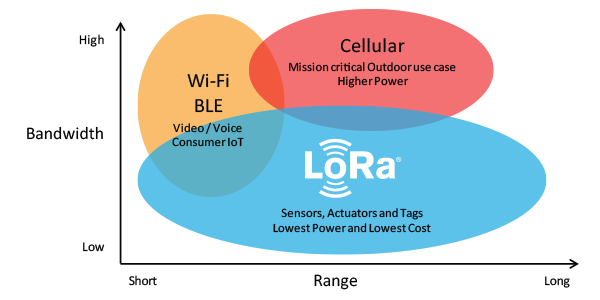
\includegraphics[width=\textwidth]{resources/img/LoRa_Why_Range}
			\caption{}
		\end{figure}
		
		
		% PAPER : LPWAN Technologies: Emerging ApplicationCharacteristics, Requirements, andDesign Considerations
		\begin{figure}
			\centering
			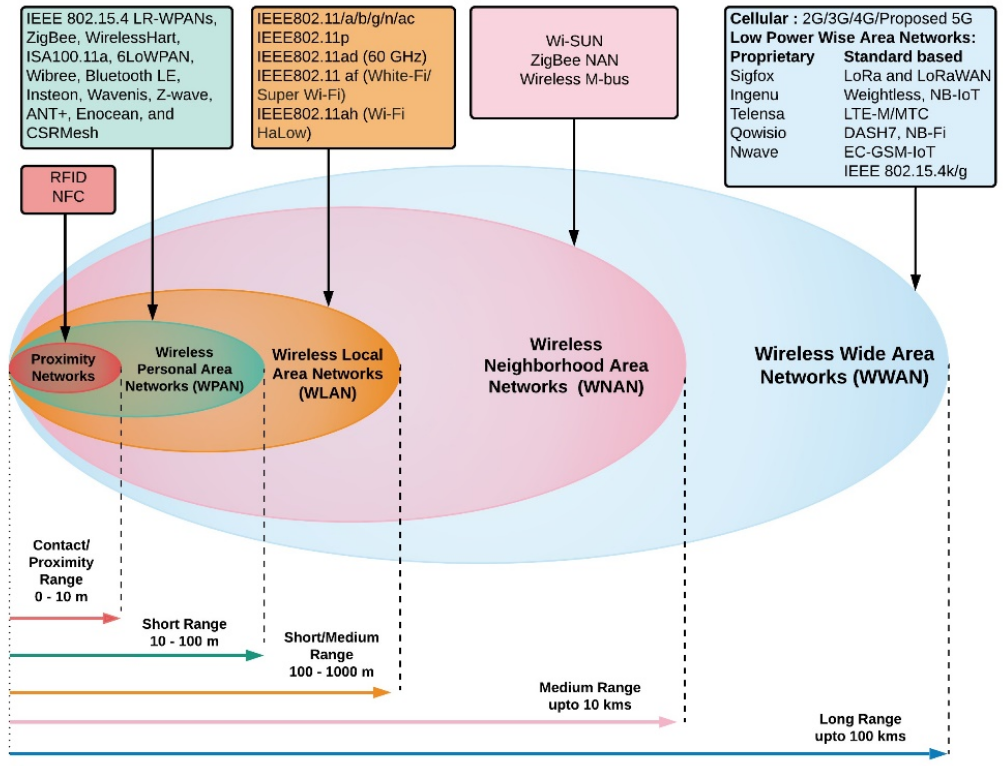
\includegraphics[height=\textwidth, angle=90]{resources/img/iot_range}
			\caption{}
		\end{figure}
	
		\subsection{LoRa}
		
		https://lora-alliance.org/
		
		https://www.semtech.com/lora
		
		\subsection{LoRaWAN}
		
		\subsection{Bluetooth}		
		
		\subsection{WiFi}
		
		IEEE 802.11, better known in the public as WiFi, short for wireless fidelity
	
		\subsection{LTE}
		
		
	
	\section{LoRa and LoRaWAN}
	
	\section{Hardware (Microcontrollers)}
	
		\subsection{Arduino}
		
		\subsection{Raspberry Pi}
		
		\subsection{Pycom}
		
			\noindent
			\begin{minipage}{0.5\textwidth}% adapt widths of minipages to your needs
				
\includegraphics[width=\textwidth]{resources/img/pycom-logo-new-rp1}
				\captionof{figure}{\textit{Pycom} company logo}
			\end{minipage}%
			\hfill%
			\begin{minipage}{0.55\textwidth}\raggedright
				Yesterday,\\
				all my troubles seemed so far away\\
				Now it looks as though they're here to stay\\
				Oh, I believe in yesterday.				Yesterday,\\
				all my troubles seemed so far away\\
				Now it looks as though they're here to stay\\
			\end{minipage}
		
		% TODO ADD TO REFERENCES
		% https://docs.pycom.io/gitbook/assets/lopy4-pinout.pdf
			